% ------------------------------------------------------------------------ %
% !TEX encoding = UTF-8 Unicode
% !TEX TS-program = pdflatex
% !TEX root = ../Tesi.tex
% !TEX spellcheck = it-IT
% ------------------------------------------------------------------------ %
%
% ------------------------------------------------------------------------ %
% 	NOME APPENDICE 2
% ------------------------------------------------------------------------ %
%
\chapter{How to calculate the ellipse's and hyperbola's coefficients}
%
\label{cap:AppendixB}
%
% ------------------------------------------------------------------------ %
%

\medskip
\section{Ellipse}
For the ellipse showed in Figure \ref{fig: System AppendixB}, the ellipse is defined as:
\begin{equation}
\left( \frac{x^{'}}{a} \right)^2 + \left( \frac{y^{'}}{b} \right)^2 = 1
\end{equation}
with
\begin{equation}
c^2 = a^2 - b^2
\end{equation}
Because the ellipse is the curve in a plane surrounding two focal points such that the sum of the distances to the two focal points is constant for every point, so:
\begin{equation}
p + q = (c + a) + (a - c) = 2 a
\end{equation}
Thus
\begin{equation}
a = \frac{p + q}{2}
\end{equation}
Now, considering the triangle $A A^{'} P $, using the law of cosines, and substituting with the equations above:
\begin{equation}
4 c^2 = p^2 + q^2 - 2 p q cos (2 \theta)
\end{equation}
\begin{equation}
4 (a^2 - b^2) = p^2 + q^2 - 2 p q cos ( 2 \theta)
\end{equation} 
\begin{equation}
(p + q)^2 - 4 b^2 = p^2 + q^2 - 2 p q cos (2 \theta)
\end{equation}
\begin{equation}
b^2 = \frac{2 p q (1 + cos (2 \theta)}{4}
\end{equation}
\begin{equation}
b = \sqrt{p q} cos (\theta)
\end{equation}
\begin{figure}[H]
%
\centering
%
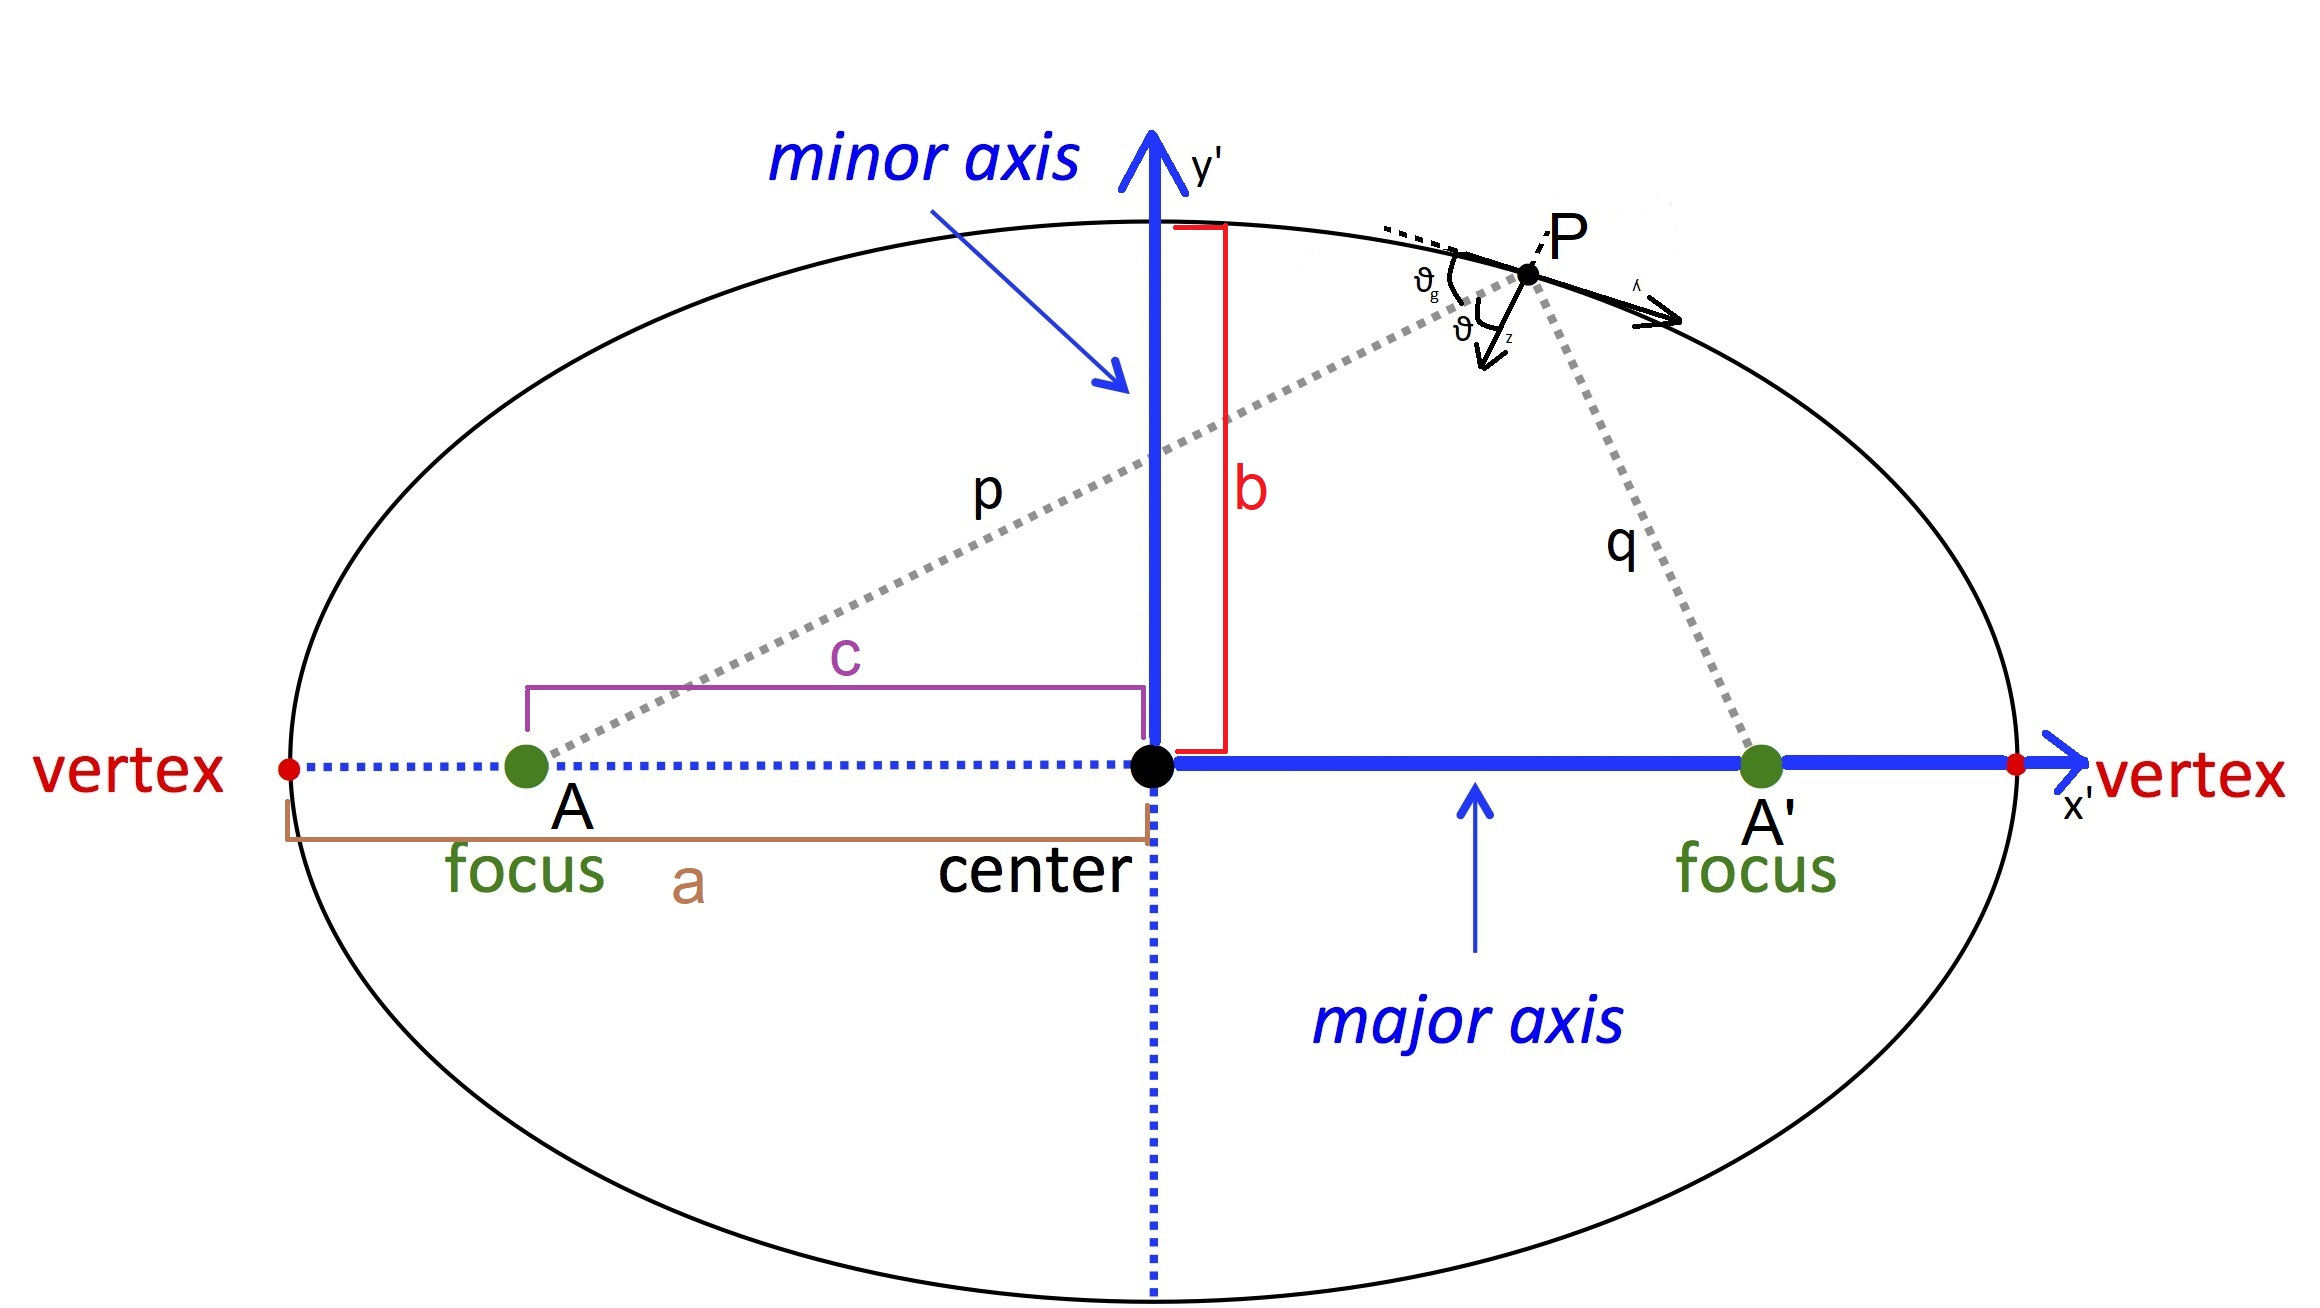
\includegraphics[width=.6\textwidth]{Immagini/AppendixB/EllipseSystem3}
%
\caption{Ellipse's system}
%
\label{fig: System AppendixB}
%
\end{figure}
\section{Hyperbola}
For the Hyperbola the situation is similar. For the system in Figure \ref{fig: System hyperbola AppendixB}, the equation of the parabola is
\begin{equation}
\left( \frac{x^{'}}{a} \right)^2 - \left( \frac{y^{'}}{b} \right)^2 = 1
\end{equation}
with
\begin{equation}
c^2 = a^2 + b^2
\end{equation}
In this case the definition of hyperbola is the curve in a plane surrounding two focal points such that the difference of the distances to the two focal points is constant for every point, so:
\begin{equation}
p - q = (c + a) - (c - a) = 2 a
\end{equation}
Thus
\begin{equation}
a = \frac{p - q}{2}
\end{equation}
As before, considering the triangle $F_1 F_2 P $, using the law of cosines, and substituting with the equations above:
\begin{equation}
4 c^2 = p^2 + q^2 - 2 p q cos (2 \theta_g)
\end{equation}
\begin{equation}
4 (a^2 + b^2) = p^2 + q^2 - 2 p q cos ( 2 \theta_g)
\end{equation} 
\begin{equation}
(p - q)^2 + 4 b^2 = p^2 + q^2 - 2 p q cos (2 \theta_g)
\end{equation}
\begin{equation}
b^2 = \frac{2 p q [1 - cos (2 \theta_g)]}{4}
\end{equation}
\begin{equation}
b = \sqrt{p q} sin (\theta_g) = \sqrt{p q} cos (\theta)
\end{equation}
\begin{figure}[H]
%
\centering
%
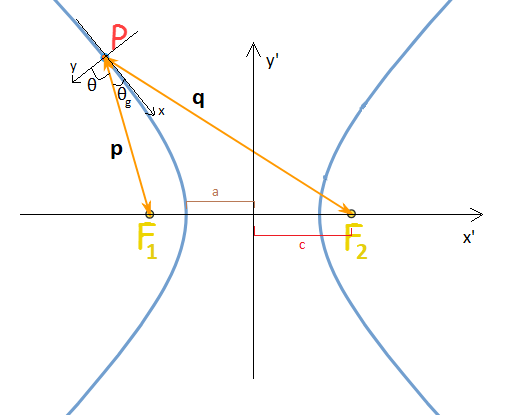
\includegraphics[width=.8\textwidth]{Immagini/AppendixB/Hyperbola}
%
\caption{Hyperbola's system}
%
\label{fig: System hyperbola AppendixB}
%
\end{figure}
